
\documentclass[12pt]{report}
\usepackage{graphicx}
\usepackage[francais]{babel}
\usepackage[utf8]{inputenc}
\usepackage[T1]{fontenc}
\usepackage{alltt}
  
\title{Rapport de soutenance \no{1}} 
\date{}
\author{TeGaSz}
\newcommand{\HRule}{\rule{\linewidth}{0.5mm}}



\begin{document}

\begin{titlepage}



\begin{center}



\textsc{\LARGE PROJET}\\[1.5cm]

\textsc{\Large TeGaSz}\\[0.5cm]


% Title
\HRule \\[0.4cm]
{ \huge \bfseries Rapport de Soutenance 1}\\[0.4cm]
  
\HRule \\[1.5cm]

\includegraphics[width=0.6\textwidth]{./name.jpg}\\[1cm]  
% Author and supervisor
\begin{minipage}{0.4\textwidth}
\begin{flushleft} \large
Julien \textsc{Garagnon}\\
Julien \textsc{Szkudlareck}
\end{flushleft}
\end{minipage}
\begin{minipage}{0.4\textwidth}
\begin{flushright} \large
Maxime \textsc{Templé}\\

\end{flushright}
\end{minipage}

\vfill

% Bottom of the page
{\large 13 mars 2012}

\end{center}

\end{titlepage}

\tableofcontents

\chapter{Le Projet}
	\section{Introduction}
Dans ce cahier des charges, nous allons vous présenter notre projet, ainsi que toute la démarche, qu'elle soit intellectuelle, sous forme de recherche ou tout simplement en code pur.
Notre projet est un logiciel de lecture audio nommé PROJET (Programme Radiophonique Oriente Jouant Enormement sur les Tonalites). Dans la suite de ce rapport, nous présenterons de façon détaillée toutes les parties que nous avons étudié. Le projet aura été développé sous et pour Fédora, en C et en Caml.

\begin{center}

\includegraphics[scale = 0.2]{logo_fedo.png}
\end{center}
\newpage

	\section{Les origines du projet}

\begin{center}

\includegraphics[scale= 0.3]{./name.jpg}\\[1cm]  
\end{center}

Le groupe\textit{ TeGaSz} est un groupe de projet formé en 2012 par trois  étudiants d'EPITA passionnés, dans le but de réaliser pour la fin de l'année un travail de programmation inédit. Ce programme est un lecteur audio codé dans la majeure partie en C et en Caml. Le projet sera accompagné d'un site web qui décrira tout au long de l'année l'avancement du projet. Il sera mis à  jour régulièrement après chaque évolution notable.
Ce projet sera particulièrement difficile à  réaliser au niveau de la programmation:
En effet, ce projet demande des notions particulièrement avancées dans le domaine du cryptage des fichiers audio. Par exemple, il faudra être capable de distinguer les en-tête de fichier de type .mp3, ou tout simplement être capable de lire un son, montrer sons avancement dans le temps, et pourquoi pas, afficher plusieurs informations sur la musique en cours.
 C'est pourquoi nous allons commencer ce projet en progressant étape par étape.

\newpage

	\section{Étude du marché}
Nous nous intéressons principalement aux lecteurs audio libres, puisque c'est à  cela que nous espérons arriver. voici quelques uns des logiciels disponibles sur le marché:

\subsubsection{The KMPlayer}

Simple et épuré KMPlayer n'en est pas moins puissant. Ce lecteur Coréen a le vent en poupe et il se dit dans les forums qu'il commence à faire de l'ombre à VLC. Lecteur multimédia, KMPlayer est capable de lire pratiquement tous les formats audio et vidéo nativement. Il est doté d'une très belle interface vraiment simple à  utiliser. A découvrir... Il est gratuit et un patch français est disponible.

\subsubsection{Amarok}

Amarok est un lecteur audio. Il était au départ conçu uniquement pour Linux, mais la migration vers les plateformes Windows et Mac OS X est en cours. C'est\`a ce jour l'un des meilleurs lecteurs audio. 
 Amarok peut lire quasiment n'importe quel type de fichiers audio (MP3, OGG, WMA, FLAC...), permet la création de playlists ce qui le transforme en Jukebox, gère l'édition des tags, grave les CD audio (à condition d'avoir K3B), récupère les pochettes de disques ou les paroles d'un morceau, permet d'uploader votre musique vers de nombreux baladeurs (iPod, Creative NOMAD ou ZEN, Rio Karma...), affiche les informations de Wikipedia sur le groupe que vous écoutez... Bref, Amarok est un outil très puissant.
Il faut disposer d'un moteur de décodage tel que GStreamer ou Xine pour faire fonctionner Amarok : Amarok est en quelque sorte une interface utilisateur. 

\subsubsection{Splayer}

Lecteur multimédia extrêmement léger, Splayer est compact, gratuit, facile à utiliser et capable de lire pratiquement tous les formats audio et vidéo sans avoir besoin de plugins supplémentaires. Il est doté d'une superbe interface que l'on apprécie d'autant plus quand on utilise Splayer pour lire des vidéos. 

\subsubsection{Windows Media Player}

Le format WMA est la réponse de Microsoft au MP3. Face au succès du MP3 et l'engouement des internautes pour ce format, Microsoft a réagi en mettant au point le Windows Media Audio codec en 1999. Les techniques de compression sont semblables à celles utilisées par le standard MP3. Windows Media Player est fourni directement avec Windows depuis Windows 98. Pour obtenir la dernière version, voyez les liens ci-dessous. Windows Media Player permet la lecture des CD audio, des fichiers MP3 et WMA et la visualisation de fichiers vidéo. Il est doté d'un égaliseur 10 bandes, d'un gestionnaire de Playlists qui le transforme en Jukebox. Il permet la compression des fichiers Wave en WMA. On peut aussi procéder à l'extraction des pistes audio d'un CD. Les fichiers obtenus sont directement encodés en WMA (on ne récupère pas les wave). Il existe des skins et des plug-ins pour le transfert vers des baladeurs.

\subsubsection{Winamp}

Premier lecteur MP3 logiciel apparu sur le Web en 1997 et toujours très populaire. Aujourd'hui, Winamp est bien plus qu'un simple lecteur MP3. Il permet la lecture des CD audio, des fichiers MP3, OGG, AAC et WMA sans ajout de plug-ins et ceci pour ne parler que des formats les plus courants. Il peut désormais ripper les pistes d'un CD audio pour les copier sur votre disque dur et graver des CD. Ces deux dernières fonctionnalités sont limitées dans la version gratuite : on peut ripper en x6 et graver en x2 seulement mais c'est possible. Cette limitation ne nous semble pas un gros handicap dans la mesure o\`u il vaut mieux ripper \`a  vitesse lente pour obtenir une bonne qualité d'extraction. Mais revenons \`a  Winamp... Il est doté d'un égaliseur 10 bandes, d'un gestionnaire de Playlists qui le transforme en Jukebox et d'un mini navigateur Web. 
L'ajout de plug-ins étend encore les possibilités de Winamp puisqu'on peut encoder en MP3 ou autre format, visualiser des vidéos au format DivX, lire des fichiers audio de type VQF, Monkey... A tester !

\newpage

\section{présentation de l'équipe}
\section{Présentation des membres de l'équipe}
		\subsection{Maxime Templé}

Il y a maintenant quatre ou cinq ans, j'ai découvert les possibilités que pouvaient donner l'informatique. Malgré quelques notions de C et depuis six mois de CaML,et un projet en C\# je n'ai jamais eu l'occasion de m'investir pleinement dans le domaine du son lié à la programmation, mais je compte me servir de ce projet afin d'approfondir mes connaissances dans le domaine.

		\subsection{Julien Garagnon}

Troisième année a l'Epita, troisième spé, et enfin je commence le C. Après l'échec du projet cartographie, j'espère bien me rattraper avec cette fois ci un groupe soudé et motivé. n'ayant pratiquement aucune expérience concernant le son, que ça soit sa lecteur, sa production ou encore sa manipulation, ce projet promet de m'apporter de nombreuses connaissances sur le sujet, connaissances dont je suis toujours avide.

		\subsection{Julien Szkudlarek}
		Après un premier projet consistant à réaliser une cartographie 3D avec un grand intérêt principalement lié à la visualisation, celui-ci sera donc un lecteur audio. Il s'annonce tout aussi passionnant car le principe même du projet est un outil très commun et de notre quotidien aujourd'hui. Il va également me permettre de pouvoir approfondir le C que je connais relativement peu. Pouvoir créer son propre lecteur audio est un objectif très stimulant d'autant plus que le sujet est plus libre que le précédent ce qui va permettre une meilleure créativité.
\newpage


\chapter{Planning et répartition des tâches}
\section{Organisation du travail} %bullshiiiiiit!!!!!!!!
		\subsection{Travail hebdomadaire}

Pour pouvoir réaliser ce projet dans les temps, nous avons choisi de travailler en groupe au moins une fois par semaine, sur des plages d'horaires communes comme le Vendredi soir ou le jeudi matin. Le reste du travail sera réalisé individuellement par chaque membre de l'équipe en suivant un planning et une répartition organisée des tâches décrite plus bas. Le but de ces réunions hebdomadaires est tout simplement de mettre en commun nos idées et de faire le point sur l'avancée du travail de chacun. Ainsi, chaque semaine un planning pour la semaine suivante sera établi pour chaque membre de l'équipe.

		\subsection{Communication entre les membres} %fake, trouver une autre idee

Pour faciliter la communication entre nous, nous avons créé un forum de développement o\`u tous nos travaux seront postés au fur et \`a  mesure de leur réalisation. Cela permettra d'une part, une meilleure gestion du travail, et d'autre part de voir l'avancement des travaux de chacun des membres. Skype sera aussi un des principaux moyens de communication.

En outre, il nous fallait un outil fiable afin de partager notre avancé commune. Le gestionnaire de version décentralisé GIT semblait tout destine pour cette tache. Pour cela, nous avons donc créé un dépôt sur le site GitHub qui permet gratuitement d'héberger l'ensemble de nos sources.

		\subsection{Chef de projet}

La personne qui s'occupera tout au long de l'année de la mise en place du projet et de l'organisation des travaux sera Maxime, choisi à l'unanimité. Il sera notre chef de projet, c'est-à-dire le principal intermédiaire entre le jury et le groupe de projet lors des soutenances.

%trois pages
\chapter{L'Interface graphique}

Pour mettre en place un projet facilement ergonomique, nous avons choisi de mettre en place une interface en utilisant GTK. deux interfaces ont été mises en place. la première, en C, pour tester les différentes fonctionnalités, et la seconde en Caml pour simplifier la tâche.
	\section {Histoire de GTK}

\begin{center}

\includegraphics[scale = 1]{GTK.png}
\end{center}

GTK+ (The GIMP Toolkit) est un ensemble de bibliothèques logicielles, c'est-à-dire un ensemble de fonctions informatiques, permettant de réaliser des interfaces graphiques. Cette bibliothèque a été développée originellement pour les besoins du logiciel de traitement d'images GIMP. GTK+ est maintenant utilisé dans de nombreux projets, dont les environnements de bureau GNOME, Xfce et ROX.
GTK+ est un projet libre (licence GNU LGPL 2.1) et multiplate-forme.

Même si, au départ GTK+ est écrit en langage C et utilise pourtant le paradigme de la programmation orientée objet. Il est également possible d'utiliser GTK+ dans de nombreux autres langages de programmation: C++ (avec gtkmm), Ada (avec GtkAda), Fortran (avec gtk-fortran), Pascal, PHP, Perl, Ruby, Objective Caml, Java, Python, Vala, Seed (JavaScript) ou encore C\# avec la plateforme mono au travers du binding Gtk\#, etc.

\section{Interface OCaml}

Pour cette dernière version, le principe de base aura été de repartir à zéro. Nous avons utilisé nos connaissances acquises dans nos recherches pour réaliser une interface qui correspondait beaucoup plus aux attentes du cahier des charges. Bien que les methodes employées pour la plupart des parties restent fondamentalement les memes, nous avons surtout ajouter des actions plus spécifiques, permettant ainsi une meilleure interconnexion entre les différentes parties du projet.

\begin{center}
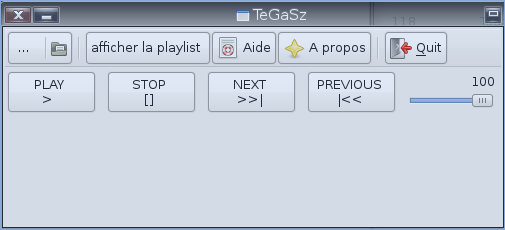
\includegraphics[scale = 0.75]{interface1.png}
\it{apercu de l'interface}
\end{center}

L'interface inclue toutes les fonctions que l'on peut attendre d'un lecteur audio basique. Nous pouvons sélectionner le fichier à charger, un bouton play permettant de lancer le fichier sélectionné, un bouton stop pour arrêter la lecture, et une barre de volume pour régler l'intensité du son. Il y a aussi deux boutons pour changer de piste, bien que ils ne soient pas encore fonctionnels.

Une des particularité du bouton de lecture est qu'il permet aussi de mettre en pause la lecture. Une fois pressé, il reste enfoncé et ainsi l'utilisateur sait que la piste est lue. S'il est de nouveau cliqué, il ressort et la lecture est mise en pause et peut être reprise au même point.

La sélection du volume se fait par une barre coulissante, avec une indication numérique du volume actuel pour une plus grande precision. A la base, le volume est indique avec une décimale, ainsi pour raison esthétique, nous avons préféré ne garder que les entiers.

\begin{center}
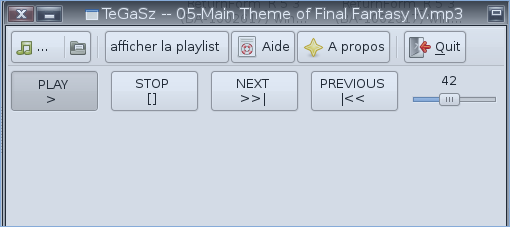
\includegraphics[scale = 0.75]{interface-volume.png}
\it{lecture d'un son avec changement de titre de fenêtre et ajustement du volume}
\end{center}

Autre détail d'ordre visuel, lors de la lecture du son, le nom du fichier est ajoute dans la barre de titre de la fenêtre. Ainsi, sans même avoir l'interface sous les yeux, il est possible de savoir quel son est joue.

Petite fonctionnalité pratique en cas de panne de pile de la souris, l'interface est entièrement utilisable au clavier via les touches de directions et la touche de tabulation.

%cinq pages
\chapter{interface C/ Caml}

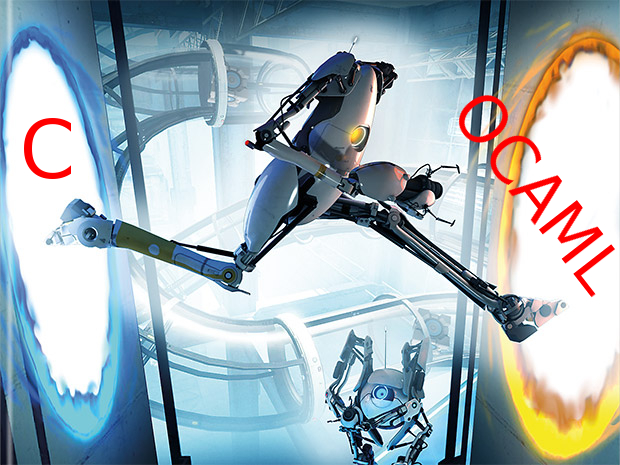
\includegraphics[scale=0.5]{COcaml.jpg}

Ce projet est soumis a une condition principale, très nouvelle pour nous : faire coexister le langage C avec le OCaml. Le partage entre les deux doit être relativement équitable tout au long du programme. En fait, lors du projet précédent nous avons déjà eu l'occasion de faire dialoguer les deux langages, via l'utilisation de GTK (écrit en C), notamment pour l'interface.\\

Ceci a donc été la principale raison qui nous a pousse a faire l'interface de ce projet-ci en Caml. L'interface entièrement en OCaml doit donc appeler des fonctions, comme la lecture d'un fichier, en C.\\

Tous les types OCaml sont exportés dans le monde C avec le type unique "value". On convertit ensuite les valeurs de ce type en données manipulables par le C, et on renvoie une valeur qui, elle aussi, doit être de type "value". Le code C et le code OCaml sont placés dans des fichiers séparés qui diffèrent par leur nom. En effet, a la compilation, deux fichiers .o seront générés ayant le même nom, un pour la version en Ocaml et l'autre en C. Ceci posera alors problème. On ne fait que appeler du C a partir du OCaml.\\

Comme il a été dit plus haut, c'est l'interface qui est codée en OCaml. C'est lorsque l'utilisateur veut lire une musique que le programme appelle une fonction en C. Le bouton "play" de l'interface, code en Ocaml, appelle une fonction en C dans un autre fichier qui va lire le fichier musical choisi.\\

L'un des problèmes majeurs auquel nous avons été confronte fut la compilation. En effet, puisque nous utilisons une libraire externe, FMOD donc, nous n'avons pas pu faire le lien directement via les commandes de compilations habituelles, notamment l'utilisation des .o, car OCamlc ne peut utiliser en même temps les .o et les .so (produit par FMOD) pour produire les exécutables. Il a donc fallu mettre notre code C dans sa propre librairie qui sert de lien avec l'OCaml, la compilation intégrant notre librairie de liens.\\

Actuellement, les fonctions stop, pause, volume et de chargement de fichier utilisent enfin le dialogue C - OCaml. En effet, elles utilisent chacune des fonctions de FMOD qui ne sont disponibles qu'en C.

%\section{Ce qu'il reste à faire}


%Pour le moment, le lecteur n'exécute que sa fonction vitale : lire un fichier de musique. Bien sur de nombreuses autres possibilités restent a inclure comme la possibilité de mettre en pause ou carrément d'arrêter la lecture. Tout cela sera géré en lien entre OCaml et le C car tout ceci sera exécutable via les boutons de l'interface.\\

\chapter{Moteur son}

\section{Le Son}


Le son est une onde produite par la vibration mécanique d'un support fluide ou solide et propagée grâce à l'élasticité du milieu environnant sous forme d'ondes longitudinales. Par extension physiologique, le son désigne la sensation auditive à laquelle cette vibration est susceptible de donner naissance.\\
\begin{center}

\includegraphics[scale=0.5]{onde.jpg}

\it{Une onde}
\end{center}

Dans un milieu compressible, le plus souvent dans l'air, le son se propage sous forme d'une variation de pression créée par la source sonore. Un haut-parleur, par exemple, utilise ce mécanisme. Seule la compression se déplace et non les molécules d'air, si ce n'est de quelques micromètres. Lorsque l'on observe des ronds dans l'eau, les vagues se déplacent mais l'eau reste au même endroit, elle ne fait que se déplacer verticalement et non suivre les vagues (un bouchon placé sur l'eau reste à la même position sans se déplacer). Le son se propage également dans les solides sous forme de vibrations des atomes appelées phonons. Là encore, seule la vibration se propage, et non les atomes qui ne font que vibrer très faiblement autour de leur position d'équilibre.\\

Le son en informatique est toujours représenté de manière numérique. De nombreux standards existent; certains s'appliquent à la production, au stockage et à la diffusion, d'autres (ceux qui utilisent des algorithmes de compression de données ou de débit), sont destinés, en principe, uniquement à la diffusion. Actuellement, le format le plus utilisé est de loin le mp3, suivi du wma, et de l'aac. C'est pourquoi nous avons décidé d'utiliser une librairie permettant de gerer de nombreux formats sonores, c'est à dire FMOD.\\


Les formats audio varient selon :\\

    Le nombre de canaux sonores encodés.\\
  Le nombre d'échantillons par seconde avec lequel on découpera numériquement, pour chaque canal, une onde sonore ou un signal électrique.\\
   La résolution donnée à chaque échantillon et la grandeur physique qu'on lui donne.\\
    l'application d'une compression ou non.\\

Chaque format audio présente aussi des caractéristiques découlant de l'algorithme de compression/décompression, ou codec (ou « codage-décodage » - COde-DECode en anglais), qu'il utilise ou non. Après la numérisation du son, le format utilisé est inscrit dans l'extension du fichier de données qui en stocke la transcription. Chaque format se caractérise aussi par sa propension à inclure et gérer des Métadonnées.\\

Dans un format donné, les fichiers peuvent être déclinés en plusieurs échelles de quantification (8, 16 ou 24 bits) avec différentes fréquences d'échantillonnage (p. ex. 22.05, 44.1, 48, 88.2 ; 96, 176.4, 192, kilohertz) appliqués à un certain nombre de voies (monophonique, stéréophonique, 5.1 surround, etc).\\

Le nombre de canaux sonores peuvent être réels et séparés, ou mélangés discrètement aux signaux principaux; ils seront décodés et restitués par la suite à l'aide d'algorithmes spécifiques (Surround).\\


\subsection{La question de la qualité}
Pour un format de fichier non compressé, la qualité peut être assez bien évaluée par le débit et la quantification mise en application. Pour un format compressé, le problème est différent : tout dépend de la performance du codec de compression (c'est-à-dire sa capacité à ne pas détruire les informations contenues dans le signal sonore tout en le compressant). En théorie, un fichier compressé avec une taille inférieure à celle d'un codage pour CD peut avoir une qualité supérieure. En pratique, d'une part on choisit souvent des compressions privilégiant trop la diminution de la taille pour que ce soit le cas, d'autre part souvent la source avant compression est un fichier CD.\\

Aidé par les nouveaux supports informatiques, le son peut être numérisé en 24 bits, voire 32 bits, contre 16 bits sur CD. Ceci permet d'améliorer le rapport signal bruit et autorise la prise de son a des niveaux plus bas.\\

La fréquence quant à elle est passée à 88.2, 96, 176.4, ou 192 kHz, contre 44.1 pour le CD.\\

Des offres de son de qualité supérieure au CD existent : pour les disques physiques, le DVD-Audio ou le SuperAudio CD de Sony, qui a l'avantage d'exister en version hybride : il est lisible à la fois selon la norme CD Audio classique, sur tous les lecteurs, et en SACD sur un lecteur dédié. Pour les offres en lignes, certains sites proposent de télécharger des musiques encodées à 96 kHz, et 24 bits.\\

Pour le grand public, ces nouveaux formats reçoivent un accueil mitigé : les audiophiles les apprécient, mais la majorité non seulement se contente de la qualité CD, mais se tourne vers les formats de compression, perdant de la qualité pour gagner en portabilité.\\

Il faut rappeler que le CD lui-même a été calibré suivant les limites de l'audition humaine normale qui se situe en moyenne entre 20 Hertz et 20 000 Hertz. La qualité supérieure n'a donc pas d'intérêt pour tous.\\

Toutefois l'utilisation de formats de qualité supérieure est indispensable durant les phases d'enregistrement et de production. La précision supplémentaire ainsi obtenue autorise des calculs plus fins lors de traitements numériques dans les logiciels audio. Ceci permet une amélioration subtile de la qualité lors de l'application d'effets tels que la réverbération.\\

\subsection{Le MP3}

Le MPEG-1/2 Audio Layer 3, plus connu sous son abréviation de MP3, est la spécification sonore du standard MPEG-1/MPEG-2, du Moving Picture Experts Group (MPEG). C'est un algorithme de compression audio (voir aussi codec) capable de réduire drastiquement la quantité de données nécessaire pour restituer de l'audio, mais qui, pour l'auditeur, ressemble à une reproduction du son original non compressé : avec une bonne compression la différence de qualité devenant difficilement perceptible.\\

L'extension de nom de fichier est .mp3 et le type MIME est audio/mpeg1, audio/MPA, audio/mpa-robust2, ou audio/mp3 (dans les navigateurs Chrome/Chromium). Ce type de fichier est appelé « fichier MP3 ».\\

Dès le début des années 2000, des réseaux d'échange sur Internet via des logiciels de partage de fichiers tels que Napster, ont beaucoup contribué à l'adoption de ce format par les consommateurs aux dépens des formats concurrents MPEG-4 Audio/TwinVQ et OGG Vorbis. Dans le même temps, les films encodés en DivX (pour la vidéo) et MP3 (pour le son) ont fait leur apparition. C'est pourquoi des constructeurs d'appareils électroniques ont commencé à commercialiser des platines lecteurs DVD-CD-DivX, des baladeurs CD Audio et des platines CD Audio capables de lire un CD de données contenant des fichiers audio MP3. Par la suite, le CD MP3 fut moins répandu avec l'apparition de baladeurs MP3 tel que l'iPod, ce qui n'améliora pas la situation du Super Audio CD et du DVD-Audio.\\

Aujourd'hui le format MP3 a été adopté par la majorité des sites de vente de musique en ligne tel que la Fnac ou Amazon. Seul l'iTunes Store vend de la musique au format MPEG-2/4 Audio/AAC. Le MP3 a aussi trouvé sa place pour les flux audio des radios en ligne et autres sites d'écoute de musique ainsi que dans les flux vidéos diffusés au format Flash (FLV encodé en VP6). La majorité des jeux PC l'utilisent. Le MP3 s'est largement imposé face à ses concurrents directs que sont les formats de compression mp3PRO, WMA, OGG Vorbis et MPEG-2/4 Audio/AAC.\\

\section{Ce qui a été fait}
Nous utilisons une librairie externe, FMOD, qui se charge de la décompressions des fichier audio et d'autre fonctions au niveau du système. Nous avons donc un "objet" principal, appelé un SoundSystem, qui gère tous les paramètres sonore. FMOD nous donne aussi des structures Sound, qui, comme on pourrais s'en douter, contiennent les informations sonores elle mêmes. On peut donc facilement associer le système et le sound afin de pouvoir jouer le son sur notre ordinateur.\\

\chapter{Ce qu'il reste a faire}

Maintenant que toutes les fonctions de base ont été implémentées (lecture, pause, arrêt, chargement), nous pourrons ajouter des fonctions pour une utilisation complète du lecteur.

L'une d'entre elle est la possibilité d'utiliser des playlist, une liste de sons qui seront joues les uns après les autres. Les boutons Next et Previous prendront alors tout leur sens. Cette fonctionnalité est présente dans tous les lecteurs modernes, il nous parait donc indispensable de l'intégrer. Vous pourrez ainsi utiliser PROJET pour toutes vos soirées sans aucun soucis. Ensuite, le lecteur devra afficher la pochette ou l'illustration du fichier lu. L'image qui aura le même nom que le fichier joue sera ouverte dans une nouvelle fenêtre.

\chapter{Site web}
Tout le squelette du site web a été mis en place. En effet nous avons très vite choisi de créer le site web en HTML, ce qui ne permettait pas de faire une interface trop esthétique. Nous avons donc tout mise sur la visibilité de l'information. La page de garde nous indique quelles sont nouveautés de l'aventure TeGaSz avec un système de news, puis trois barres, indiquant notre progression dans le projet. \\
Une autre page explique avec précision ce qu'est exactement TGgaSz et comment l'avons nous implémenté. nous avons bien sûr une page destinée à la présentation du groupe de projet , chaque personne se décrivant brièvement et expliquant son rôle dans le projet. vient ensuite une page ``livre d'or'' permettant a tout utilisateur du projet de donner son avis sur le site et des commentaire des remarques, ou des demandes... Enfin, un dernier bouton permet d'envoyer un mail aux programmeurs pour des questions particulières.\\
 Ce site ce veut être une vitrine pour le projet et veut donner envie aux utilisateurs de l'utiliser.

\chapter{Conclusion}

Dans ce rapport qui présente de façon détaillée notre projet de logiciel de lecteur audio nomme Projet Radiophonique Oriente Jouant Énormément sur les Tonalités (PROJET), nous avons pu nous rendre compte de l'avancement rapide du logiciel. Toutes les fonctionnalités vitales d'un lecteur basique sont en place et fonctionnelles. Le développement du projet est dans les temps du planning et nous sommes impatients de le finaliser avec de nouvelles fonctionnalités.

\end{document}
